\documentclass{article}

\usepackage[most]{tcolorbox}

\usepackage{microtype}
\usepackage{hyperref}
\usepackage{xcolor}
\usepackage{tikz}
\usepackage{amsmath}
\usepackage{pgfplots}
\usepackage{float}
\usepackage{fontspec}
\setmonofont{Consolas}

\setmainfont{Heuristica}
\usepackage[legalpaper, margin=1in]{geometry}

\hypersetup{
    colorlinks,
    linkcolor={red!50!black},
    citecolor={blue!50!black},
    urlcolor={blue!80!black}
    }
\usepackage[capitalize,nameinlink,noabbrev]{cleveref}
\usepackage{etoolbox}
\usepackage{booktabs}
\usepackage[cache=false]{minted}
    
\usepackage{varwidth}
\newtcolorbox{mybox}[2][]{enhanced,
before skip=2mm,after skip=2mm, colback=black!5,colframe=black!50,boxrule=0.2mm,
attach boxed title to top left={xshift=1cm,yshift*=1mm-\tcboxedtitleheight}, varwidth boxed title*=3cm,
boxed title style={frame code={
            \path[fill=tcbcolback!30!black]
              ([yshift=-1mm,xshift=-1mm]frame.north west)
                arc[start angle=0,end angle=180,radius=1mm]
              ([yshift=-1mm,xshift=1mm]frame.north east)
                arc[start angle=180,end angle=0,radius=1mm];
            \path[left color=tcbcolback!60!black,right color=tcbcolback!60!black,
              middle color=tcbcolback!60!black]
              ([xshift=-2mm]frame.north west) -- ([xshift=2mm]frame.north east)
              [rounded corners=1mm]-- ([xshift=1mm,yshift=-1mm]frame.north east)
              -- (frame.south east) -- (frame.south west)
              -- ([xshift=-1mm,yshift=-1mm]frame.north west)
              [sharp corners]-- cycle;
            },interior engine=empty,
          },
          fonttitle=\bfseries,
          title={#2},#1}
          
\BeforeBeginEnvironment{mybox}{\vspace{0.5\baselineskip}}%
\AfterEndEnvironment{mybox}{\vspace{0.5\baselineskip}}%
% \BeforeBeginEnvironment{minted}{\begin{mybox}[colbacktitle=green]{Python}}%
% \AfterEndEnvironment{minted}{\end{mybox}}%

\setlength{\parindent}{0pt}

\begin{document}

\text{\Huge Mirador Analytics - Data Science Task}

\section{k - Anonymity Analysis}


\textbf{a) Randomly generate a dataset (dataframe) with eight columns and 50,000 rows. Each column should be a categorical variable (of arbitrary name) with three levels (of arbitrary names) in approximately equal proportions.}

\vspace{\baselineskip} 

We first define a dictionary, whose keys and values will be used to generate the dataframe.
Then, using \texttt{numpy.random.choice} we can sample 50,000 times (with replacement) from the dictionary values and assign the sample to the dataframe using the dictionary keys as the column names. To ensure that the sample is repeatable, we also fix the random seed.

\begin{mybox}[colbacktitle=green]{Creating the DataFrame}
    \begin{minted}[gobble=8, breaklines]{python}
        import pandas as pd
        import numpy as np

        dictionary = dict({
            'A':['a1','a2','a3'],
            'B':['b1','b2','b3'],
            'C':['c1','c2','c3'],
            'I':['i1','i2','i3'],
            'J':['j1','j2','j3'],
            'K':['k1','k2','k3'],
            'X':['x1','x2','x3'],
            'Y':['y1','y2','y3']
        })

        np.random.seed(92)

        def categorical_df_from_dict(d: dict, size: int) -> pd.DataFrame:
            """Creates a dataframe with columns = d.keys, where each column is populated with values randomly sampled from d.values."""

            df = pd.DataFrame()

            for key, val in d.items():

                df[key] = np.random.choice(val, size)

            return df

        df = categorical_df_from_dict(dictionary, size=50000)
    \end{minted}
\end{mybox}

The first five rows of the resulting dataframe can be seen in \cref{tbl:df_head}.

\begin{table}[htbp!]
    \centering
    \caption{The first five rows of the dataframe \texttt{df}.}
    
    \vspace{0.5\baselineskip}
    \begin{tabular}{@{}llllllll@{}}
        \toprule
        A                              & B                              & C                              & I                              & J                              & K                              & X                              & Y                              \\ \midrule
        a3                             & b2                             & c3                             & i1                             & j3                             & k3                             & x3                             & y1                             \\
        a3                             & b1                             & c3                             & i2                             & j1                             & k3                             & x1                             & y2                             \\
        a1                             & b1                             & c3                             & i3                             & j2                             & k3                             & x1                             & y3                             \\
        a2                             & b3                             & c2                             & i1                             & j1                             & k1                             & x1                             & y1                             \\
        a2                             & b3                             & c3                             & i2                             & j1                             & k3                             & x1                             & y1                             \\ \bottomrule
    \end{tabular}
    \label{tbl:df_head}
\end{table}

\textbf{b) Verify that the proportions of each value are similar for each of the eight columns.}

\vspace{\baselineskip}

    
Since the values are sampled with equal probability, we expect the distribution of the samples to be uniform. That is, we should see approximately 33\% representation of each variable. This can be confirmed by looping over the columns in \texttt{df}, counting the unique values and dividing by the length of \texttt{df}.

\begin{table}[H]
    \caption{Representation of variables in each column}
    \label{tbl:props}
    \vspace{0.5\baselineskip}
    \begin{tabular}{l|llllllll}
        & a       & b       & c       & i       & j       & j       & x       & y       \\ \midrule
        1 & 0.33394 & 0.33356 & 0.33194 & 0.33266 & 0.33590 & 0.33884 & 0.33333 & 0.33054 \\
        2 & 0.33490 & 0.33686 & 0.33228 & 0.33426 & 0.33598 & 0.32884 & 0.32944 & 0.33614 \\
        3 & 0.33116 & 0.32958 & 0.33578 & 0.33308 & 0.32812 & 0.33232 & 0.33756 & 0.33332
    \end{tabular}
\end{table}

\cref{tbl:props} shows the proportions of each variable and was obtained by collecting the output of the code below.

\begin{mybox}[colbacktitle=green]{Verifying Proportions}
    \begin{minted}[gobble=8]{python}
        def verify_proportions(df: pd.DataFrame) -> None:
            """Prints the proportions of values in all columns in the dataframe df."""

            for col in df:
                vals, counts = np.unique(df[col], return_counts=True)

                print(vals)
                print(counts/sum(counts))

        verify_proportions(df)
    \end{minted}
\end{mybox}





\textbf{c) How many unique rows (i.e., permutations of category levels) are possible?}

\vspace{\baselineskip}

There are 6561 possible permutations, given by $n^r$, where $n$ is the number of unique values in each column and $r$ is the number of columns. Note that this only holds when there are an equal number of unique values in each column. A more general solution would be to use an n-fold cartesian product, which we make use of below to print the first five permutations. 

\begin{mybox}[colbacktitle=green]{Displaying Permutations}
    \begin{minted}[gobble=8, breaklines]{python}
        import itertools

        def print_permutations(n: int) -> None:
            """Prints the first n permutations from itertools.product."""

            for num, perm in enumerate(itertools.product('123', repeat=8)):
                perm = list(perm)
                letters = ['a','b','c','i','j','k','x','y']
                for x, y in enumerate(perm):
                    perm[x] = letters[x]+y
                print(perm)
                if num >= n-1:
                    break

        print_permutations(n=5)
    \end{minted}
\end{mybox}

Executing the above code results in the following output:
\begin{verbatim}
                    ['a1', 'b1', 'c1', 'i1', 'j1', 'k1', 'x1', 'y1']
                    ['a1', 'b1', 'c1', 'i1', 'j1', 'k1', 'x1', 'y2']
                    ['a1', 'b1', 'c1', 'i1', 'j1', 'k1', 'x1', 'y3']
                    ['a1', 'b1', 'c1', 'i1', 'j1', 'k1', 'x2', 'y1']
                    ['a1', 'b1', 'c1', 'i1', 'j1', 'k1', 'x2', 'y2']
\end{verbatim}

\vspace{\baselineskip}

\textbf{d) Produce a table and appropriate graph which show the frequencies (numbers of groups) by permutation group sizes up to group size of 12. That is, how many groups are unique combinations (group size = 1), how many groups are made up of a pair of matching combinations (group size = 2), how many groups are made up three the same, etc? }

\vspace{\baselineskip}

First, let's compute the frequencies of each permutation using \texttt{.groupby()} and \texttt{.size()}, then remove any where the group size is greater than 12 using \texttt{.query()}. 

\begin{mybox}[colbacktitle=green]{Creating the Frequency Table}
    \begin{minted}[gobble=8, breaklines]{python}
        unique_perms = (df
            .groupby(df.columns.tolist(), as_index=False)
            .size()
            .query('size <= 12')
        )
        display(unique_perms.groupby('size').count().iloc[:,0])
    \end{minted}
\end{mybox}

This gives us all unique permutations in \texttt{df}, with an extra column \texttt{size}, recording how many times each permutation was observed. Grouping again by size and counting the values gives us the frequencies seen in \cref{tbl:frequency}.

\begin{table}[H]
    \centering
    \caption{Size frequency table}
    \label{tbl:frequency}
    \begin{tabular}{@{}cc@{}}
    \toprule
    Group Size & No of Groups \\ \midrule
    1          & 24           \\
    2          & 122          \\
    3          & 220          \\
    4          & 453          \\
    5          & 625          \\
    6          & 863          \\
    7          & 974          \\
    8          & 989          \\
    9          & 766          \\
    10         & 580          \\
    11         & 398          \\
    12         & 230          \\ \bottomrule
    \end{tabular}
\end{table}

% \begin{table}[H]
%     \centering
%     \caption{Size frequency table}
%     \begin{tabular}{@{}cccccccccc@{}}
%         \toprule
%            & A      & B      & C      & I      & J      & K      & X      & Y      & size   \\ \midrule
%     0      & a1     & b3     & c3     & i1     & j3     & k3     & x2     & y1     & 12     \\
%     1      & a1     & b3     & c1     & i3     & j2     & k2     & x2     & y3     & 12     \\
%     2      & a3     & b2     & c2     & i1     & j1     & k3     & x1     & y3     & 12     \\
%     3      & a2     & b3     & c1     & i2     & j1     & k3     & x3     & y2     & 12     \\
%     % 4      & a2     & b3     & c1     & i1     & j3     & k3     & x2     & y3     & 12     \\
%     \vdots & \vdots & \vdots & \vdots & \vdots & \vdots & \vdots & \vdots & \vdots & \vdots \\
%     % 6239   & a2     & b3     & c3     & i3     & j1     & k1     & x3     & y3     & 1      \\
%     6240   & a2     & b1     & c2     & i2     & j3     & k1     & x2     & y1     & 1      \\
%     6241   & a1     & b3     & c2     & i1     & j1     & k3     & x2     & y3     & 1      \\
%     6242   & a1     & b1     & c2     & i2     & j2     & k1     & x2     & y3     & 1      \\
%     6243   & a1     & b1     & c2     & i1     & j3     & k1     & x2     & y2     & 1     \\ \bottomrule
%     \end{tabular}
% \end{table}

From this we can produce the histogram displayed in \cref{fig:frequency_histogram}.

\begin{figure}[H]
    \centering
    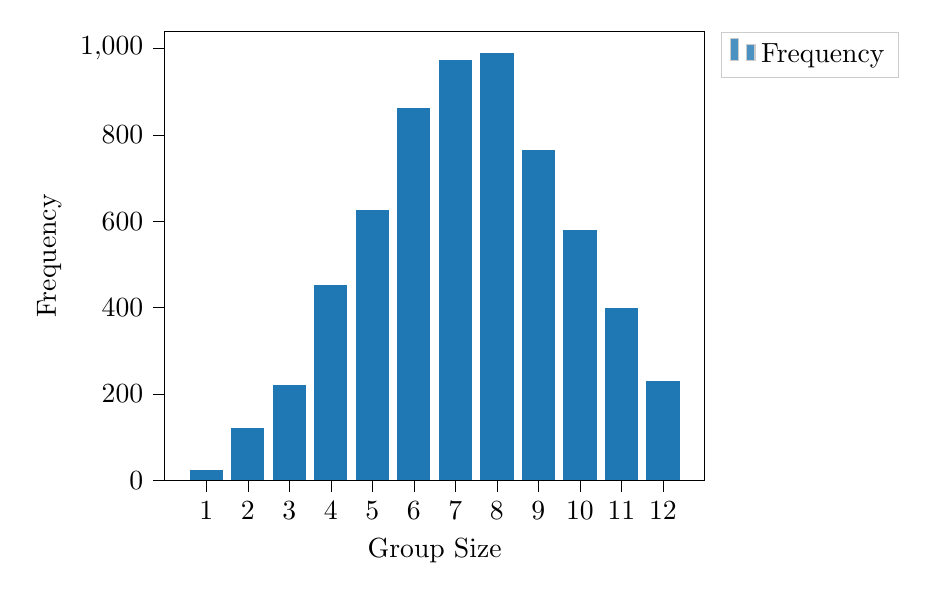
\begin{tikzpicture}
        
        \definecolor{color0}{rgb}{0.12156862745098,0.466666666666667,0.705882352941177}
        
        \begin{axis}[
            legend cell align={left},
            legend pos=outer north east,
            legend style={fill opacity=0.8, draw opacity=1, text opacity=1, draw=white!80!black},
            tick align=outside,
            tick pos=left,
            x grid style={white!69.0196078431373!black},
            xlabel={Group Size},
            xmin=0, xmax=13,
            xtick style={color=black},
            xtick = {1,2,3,4,5,6,7,8,9,10,11,12},
            xticklabel style={rotate=0},
            y grid style={white!69.0196078431373!black},
            ylabel={Frequency},
            ymin=0, ymax=1038.45,
            ytick style={color=black}
            ]
            \addlegendimage{ybar,ybar legend,draw=none,fill=color0};
            \addlegendentry{Frequency}
            \draw[draw=none,fill=color0] (axis cs:0.6,0) rectangle (axis cs:1.4,24);
            \draw[draw=none,fill=color0] (axis cs:1.6,0) rectangle (axis cs:2.4,122);
            \draw[draw=none,fill=color0] (axis cs:2.6,0) rectangle (axis cs:3.4,220);
            \draw[draw=none,fill=color0] (axis cs:3.6,0) rectangle (axis cs:4.4,453);
            \draw[draw=none,fill=color0] (axis cs:4.6,0) rectangle (axis cs:5.4,625);
            \draw[draw=none,fill=color0] (axis cs:5.6,0) rectangle (axis cs:6.4,863);
            \draw[draw=none,fill=color0] (axis cs:6.6,0) rectangle (axis cs:7.4,974);
            \draw[draw=none,fill=color0] (axis cs:7.6,0) rectangle (axis cs:8.4,989);
            \draw[draw=none,fill=color0] (axis cs:8.6,0) rectangle (axis cs:9.4,766);
            \draw[draw=none,fill=color0] (axis cs:9.6,0) rectangle (axis cs:10.4,580);
            \draw[draw=none,fill=color0] (axis cs:10.6,0) rectangle (axis cs:11.4,398);
            \draw[draw=none,fill=color0] (axis cs:11.6,0) rectangle (axis cs:12.4,230);
        \end{axis}   
    \end{tikzpicture}
    \caption{A histogram of the group size frequencies.}
    \label{fig:frequency_histogram}
\end{figure}

The code to produce \cref{fig:frequency_histogram} is below:
\begin{mybox}[colbacktitle=green]{Creating the Frequency Plot}
    \begin{minted}[gobble=8, breaklines]{python}
        import matplotlib.pyplot as plt

        sizes = unique_perms.loc[:, 'size']

        def plot_frequency_hist(x: pd.Series) -> tuple:
            """Creates the frequency histogram plot of the series x.""" 

            fig, ax = plt.subplots(1, 1, figsize=(10,5))

            # define bins and binwidth
            bins = np.arange(min(x.unique()), min(x.unique()) + len(x.unique()) + 1)
            binwidth = 0.8

            # plot hist
            plt.hist(x.values, bins=bins-0.5*binwidth, width=binwidth)

            # formatting
            ax.set_xlabel('Group Size'); ax.set_ylabel('Frequency')
            ax.set_xlim([min(x.unique()) - 1, min(x.unique()) + len(x.unique())])
            ax.set_xticks(bins[:-1])
            ax.set_xticklabels(labels=bins[:-1],rotation=45)

            return fig, ax

        fig, ax = plot_frequency_hist(sizes)

        plt.show()
    \end{minted}
\end{mybox}

\newpage

\textbf{e) Comment upon the distribution of group sizes in d). }

\vspace{\baselineskip}

This particular sample appears to follow a zero-truncated poisson distribution with a slight positive skew (obscured by the removal of sizes > 12). The distribution can be approximated using the normal distribution as shown in \cref{fig:density_plot}. 


\begin{figure}[H]
    \centering
    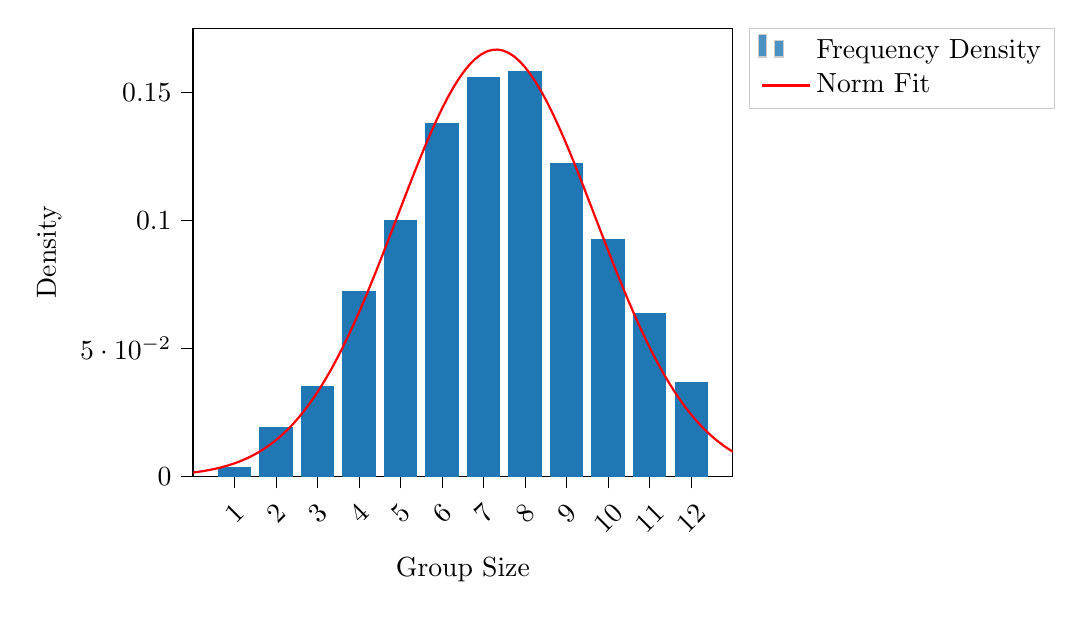
\begin{tikzpicture}

    \definecolor{color0}{rgb}{0.12156862745098,0.466666666666667,0.705882352941177}
    
    \begin{axis}[
        legend cell align={left},
        legend pos=outer north east,
        legend style={fill opacity=0.8, draw opacity=1, text opacity=1, draw=white!80!black},
        tick align=outside,
        tick pos=left,
        x grid style={white!69.0196078431373!black},
        xlabel={Group Size},
        xmin=0, xmax=13,
        xtick = {1,2,3,4,5,6,7,8,9,10,11,12},
        xtick style={color=black},
        xticklabel style={rotate=45.0},
        y grid style={white!69.0196078431373!black},
        ylabel={Density},
        ymin=0, ymax=0.175199363465411,
        ytick style={color=black}
    ]
        \draw[draw=none,fill=color0] (axis cs:0.6,0) rectangle (axis cs:1.4,0.00384368994234465);
        \addlegendimage{ybar,ybar legend,draw=none,fill=color0};
        \addlegendentry{Frequency Density}
        
        \draw[draw=none,fill=color0] (axis cs:1.6,0) rectangle (axis cs:2.4,0.0195387572069186);
        \draw[draw=none,fill=color0] (axis cs:2.6,0) rectangle (axis cs:3.4,0.0352338244714926);
        \draw[draw=none,fill=color0] (axis cs:3.6,0) rectangle (axis cs:4.4,0.0725496476617553);
        \draw[draw=none,fill=color0] (axis cs:4.6,0) rectangle (axis cs:5.4,0.100096092248559);
        \draw[draw=none,fill=color0] (axis cs:5.6,0) rectangle (axis cs:6.4,0.13821268417681);
        \draw[draw=none,fill=color0] (axis cs:6.6,0) rectangle (axis cs:7.4,0.155989750160154);
        \draw[draw=none,fill=color0] (axis cs:7.6,0) rectangle (axis cs:8.4,0.158392056374119);
        \draw[draw=none,fill=color0] (axis cs:8.6,0) rectangle (axis cs:9.4,0.122677770659833);
        \draw[draw=none,fill=color0] (axis cs:9.6,0) rectangle (axis cs:10.4,0.0928891736066624);
        \draw[draw=none,fill=color0] (axis cs:10.6,0) rectangle (axis cs:11.4,0.0637411915438821);
        \draw[draw=none,fill=color0] (axis cs:11.6,0) rectangle (axis cs:12.4,0.0368353619474696);
        \addplot [thick, red]
        table {%
        0 0.00156925159869111
        0.133333333333333 0.00185785856134929
        0.266666666666667 0.00219271357983408
        0.4 0.00257988504045417
        0.533333333333333 0.00302599350879828
        0.666666666666667 0.00353821989123075
        0.8 0.00412430559320438
        0.933333333333333 0.0047925432896303
        1.06666666666667 0.00555175690661647
        1.2 0.00641126943282341
        1.33333333333333 0.00738085723773946
        1.46666666666667 0.00847068967812905
        1.6 0.00969125292681034
        1.73333333333333 0.0110532571628359
        1.86666666666667 0.0125675265208894
        2 0.0142448715105601
        2.13333333333333 0.016095943981662
        2.26666666666667 0.0181310751264995
        2.4 0.0203600974684443
        2.53333333333333 0.0227921522806417
        2.66666666666667 0.0254354843991999
        2.8 0.0282972269297398
        2.93333333333333 0.0313831788806529
        3.06666666666667 0.0346975792750421
        3.2 0.0382428817789776
        3.33333333333333 0.0420195343183278
        3.46666666666667 0.0460257685216389
        3.6 0.0502574041041793
        3.73333333333333 0.0547076734811453
        3.86666666666667 0.0593670719505787
        4 0.0642232387056026
        4.13333333333333 0.069260873711021
        4.26666666666667 0.0744616951047551
        4.4 0.0798044412578893
        4.53333333333333 0.0852649209508742
        4.66666666666667 0.0908161143053168
        4.8 0.0964283261635553
        4.93333333333333 0.102069392549769
        5.06666666666667 0.107704939699412
        5.2 0.113298693935437
        5.33333333333333 0.118812839430838
        5.46666666666667 0.124208419661319
        5.6 0.129445777154801
        5.73333333333333 0.134485025022453
        5.86666666666667 0.139286542744676
        6 0.143811487819053
        6.13333333333333 0.148022314186661
        6.26666666666667 0.151883287865099
        6.4 0.155360989952445
        6.53333333333333 0.158424797141283
        6.66666666666667 0.161047330103926
        6.8 0.163204860579692
        6.93333333333333 0.164877668705177
        7.06666666666667 0.166050343064274
        7.2 0.166712017073742
        7.33333333333333 0.166856536633725
        7.46666666666667 0.166482555425839
        7.6 0.165593555794981
        7.73333333333333 0.164197794761856
        7.86666666666667 0.162308176336815
        8 0.159942052896464
        8.13333333333333 0.157120959898764
        8.26666666666667 0.153870289608316
        8.4 0.150218910743823
        8.53333333333333 0.146198742011949
        8.66666666666667 0.141844288329946
        8.8 0.137192149144506
        8.93333333333333 0.132280508614675
        9.06666666666667 0.127148617538779
        9.2 0.12183627677293
        9.33333333333333 0.116383331523123
        9.46666666666667 0.110829185312228
        9.6 0.105212341651121
        9.73333333333333 0.0995699805086277
        9.86666666666667 0.0939375756102936
        10 0.088348557436273
        10.1333333333333 0.0828340255699492
        10.2666666666667 0.0774225128074567
        10.4 0.0721398022088907
        10.5333333333333 0.0670087970872341
        10.6666666666667 0.0620494428201696
        10.8 0.057278698358226
        10.9333333333333 0.0527105544107377
        11.0666666666667 0.0483560945345454
        11.2 0.0442235947397151
        11.3333333333333 0.0403186567671844
        11.4666666666667 0.0366443698856324
        11.6 0.0332014958949237
        11.7333333333333 0.0299886720030994
        11.8666666666667 0.0270026263515066
        12 0.0242384011839635
        12.1333333333333 0.0216895789744715
        12.2666666666667 0.019348507226208
        12.4 0.0172065181140206
        12.5333333333333 0.0152541396450832
        12.6666666666667 0.0134812955400621
        12.8 0.0118774915734846
        12.9333333333333 0.0104319866419547
        13.0666666666667 0.00913394733920958
        13.2 0.00797258529662162
        };
        \addlegendentry{Norm Fit}
    \end{axis}
    \end{tikzpicture}
    \caption{A gaussian fitted to the frequency density of group sizes.}
    \label{fig:density_plot}
\end{figure}   

\begin{mybox}[colbacktitle=green]{Creating a Frequency Density Plot and Fitting a Distribution}
    \begin{minted}[gobble=8, breaklines]{python}
        import scipy.stats as st

        def hist_fit(x: pd.Series, dists: list) -> tuple:
            """Creates density histogram and fits the distributions in dists.""" 

            fig, ax = plt.subplots(1, 1, figsize=(10,5))

            # define bins and binwidth
            bins = np.arange(min(x.unique()), min(x.unique()) + len(x.unique()) + 1)
            binwidth = 0.8

            # plot density
            ax.hist(x.values, bins=bins - 0.5*binwidth, width=binwidth, density=True, label='Frequency Density')

            for dist_name in dists:
                xmin, xmax = ax.get_xlim()
                xx = np.linspace(xmin, xmax, 100)

                dist = getattr(st, dist_name)
                params = dist.fit(x)

                p = dist.pdf(xx, *params)
                ax.plot(xx, p, linewidth=2, label=dist_name.title() + ' Distribution Fit')

            # formatting
            ax.set_xlabel('Group Size')
            ax.set_ylabel('Density')
            ax.set_xlim([min(x.unique()) - 1, min(x.unique()) + 1 + len(x.unique())])
            ax.set_xticks(bins[:-1])
            ax.set_xticklabels(labels=bins[:-1], rotation=45)
            plt.legend()

            return fig, ax

        # experiment with other continuous distributions by adding them to the list
        fig, ax = hist_fit(sizes, dists=['norm'])

        plt.show()
    \end{minted}
\end{mybox}

\newpage 

\textbf{f) If your random variables were, in fact, meaningful information on individuals, which group sizes are of most concern from a privacy perspective?} 

\vspace{\baselineskip}

Since the goal of $k$-anonymity is to maximise $k$, we should be most concerned about the smaller group sizes, as it would be easier to match the variables to a specific individual or group of individuals. 

\vspace{\baselineskip}

\textbf{g) Consider the effect of missing data in the dataset you created in Part a). How might this complicate the production of a frequency table of group sizes in Part d)?} 

\vspace{\baselineskip}

The effect of missing data is something that we can test for quite easily by creating a function to randomly assign \texttt{np.nan} to values in our categorical dataframe. A function to do this is given below and replaces 20\% by default. 

\begin{mybox}[colbacktitle=green]{Creating Missing Values}
    \begin{minted}[gobble=8, breaklines]{python}
        def create_missing_values(df: pd.DataFrame, pct_missing: float=0.2) -> pd.DataFrame:
            """ Chooses random rows and columns and replaces the values with np.nan until the desired portion of missing data is met. """

            n = int(pct_missing*df.shape[0]*df.shape[1])

            # define all possible row/column index combinations
            all_rc_pairs = np.array(list(itertools.product(range(0,len(df)), range(0,8))))

            # randomly select a subset of size n (no replacement)
            idx = np.random.choice(len(all_rc_pairs), replace=False, size=n)
            subset_rc_pairs = all_rc_pairs[idx]

            # replace with np.nan
            for x, y in subset_rc_pairs:
                df.iat[x, y] = np.nan

            return df
    \end{minted}
\end{mybox}

Re-applying the process described in 1. d) we observe that \texttt{np.nan} values are removed by default during the \texttt{.groupby()} step. This leaves us with fewer unique permutations and smaller group sizes. Alternatively, setting \texttt{dropna=False} introduces a fourth option for each column, which in turn increases the total number of unique combinations but lowers the probability of seeing the same permutation more than once, again leading to smaller group sizes. 
The existence of these pseudo-group sizes is undesireable, as any individuals that were legitimately at risk of having their privacy compromised are now buried amongst the new cases with low group size, making it more difficult to properly assess the anonymity of the data. 

\vspace{\baselineskip}

\textbf{h) Imagine the code that you wrote for Part d) was to be deployed in an automated system that Mirador's customers could use independently, on potentially large volumes of their own data. Describe how you might deploy the code, and what additional considerations you might have or any changes to the code you might make. Note: it is not necessary to provide another version of the code created for d).}


\vspace{\baselineskip}

% \subsubsection*{Deployment}

If the customers are to use the tool independently then there are a number of deployment options. For example, you could create a GUI (PyQt, tkinter), or dashboard (Plotly/Dash), or if the end user is expected to have a technical background then you could supply a \texttt{requirements.txt} file, or Docker environment and have them run a script manually. 
Ideally, clear and easy-to-follow documentation on how to use the tool would also be supplied.\\

% \subsubsection*{Additional Pre-Processing}

We'd have to enforce a list of acceptable data formats e.g. \texttt{.csv}, \texttt{.xlsx}, and consider the possibility that the data will contain non-categorical variables such as height or weight. 
If such values are allowed, then the software will highlight to the user that their data has severe privacy concerns, as continuous values are much more likely to be unique, resulting in a low $k$-value.
The alternative is to filter them out or educate the client in binning the variables or removing them entirely prior to analysis. \\

% \subsubsection*{Processing Speed}

With regards to processing speed, assuming that we're no longer filtering out group sizes > 12, as a minimum we could re-run our code with more samples and measure the time it takes to produce the frequency table and graph. This would test its ability to process larger volumes of data. \cref{tbl:times} below shows the typical times we could expect, running on an Intel i9 9900k @ 5 GHz. However, without knowing the time constraints and dimensions of the data we're dealing with it would be difficult to comment on whether these speeds are fast enough. If the software is expected to be run locally on the client's computer, then it would be worth re-testing on a lower-spec machine. 

\begin{table}[H]
    \centering
    \caption{Computation times (seconds) for different sample sizes (thousands).}
    \label{tbl:times}
    \begin{tabular}{@{}ccc@{}}
    \toprule
    Samples (k) & Time to Filter (s) & Time to Plot (s) \\ \midrule
    50          & 0.5                & 0.1              \\
    500         & 0.2                & 0.9              \\
    5000        & 2.1                & 2.3              \\
    50000       & 52                 & 7.1              \\ \bottomrule
    \end{tabular}
\end{table}

As you increase the number of samples in the data, you increase the probability of seeing more unique group sizes.
This will become a problem when plotting the frequency histogram, as each group size is currently represented as a single bar on the chart and too many would flood the chart leading to overlapping xticklabels. 
To solve this we may want to implement an automated system to bin the higher group sizes, as it's the smaller ones we're most interested in. \\ 


It would also be beneficial to write some unit tests to import some sample files, checking that everything is computed and displayed correctly. This would help to ensure that the core functionality of the system remains in tact, should any changes be made to the code at a later date.

\section{Postcodes and Privacy}

\textbf{In the US, 5-digit Zip codes are usually rounded to 3-digits when anonymizing health data, so knowledge of the Zip code doesn't allow small groups to be identified. Even then, there are some 3-digit codes that have fewer than 20,000 residents, and the advice is to lump these together under a new code (000).} \\ 

\textbf{Looking forward to how GDPR may affect data handling in the UK, might a similar approach be possible here? In answering this, use the data below. You might want to include some examples of any postcodes which could be problematic. Write it up as a mini report to inform the decision of a privacy offcer.} \\ 

\textbf{UK population by postcode data (28 MB) found here:} \\ 

\url{www.nomisweb.co.uk/output/census/2011/Postcode_Estimates_Table_1.csv.}

\vspace{\baselineskip}

In the UK, postcodes are alphanumeric with lengths ranging from six to eight characters (including a space). The postcode is divided into two parts separated by a single space: the outward code and the inward code respectively. The outward code includes the area and district, and the inward code contains the sector and unit. Some examples of UK postcodes and their structure can be seen in \cref{tbl:postcode_structure}.

\begin{table}[H]
    \centering
    \caption{Structure of UK postcodes, with examples.}
    \label{tbl:postcode_structure}
    \vspace{0.5\baselineskip}
    \begin{tabular}{|c|c|c|c|}
        \hline
        \multicolumn{4}{|c|}{Postcode}                                        \\ \hline
        \multicolumn{2}{|c|}{Outward code} & \multicolumn{2}{c|}{Inward code} \\ \hline
        Area           & District          & Sector           & Unit          \\ \hline
        TD             & 6                & 9                & EF            \\ \hline
        AL             & 10                & 0                & AB            \\ \hline
        B             & 1                & 1                & BA            \\ \hline
        \end{tabular}
\end{table}

The following subsections will cover two possible ways to anonymize UK postcodes: the outward code and the area.

\subsection{Area Code} \label{sec:area_code}

We will perform our analysis of the postcodes using Python, starting by importing the file.


\begin{mybox}[colbacktitle=green]{Importing the CSV}
    \begin{minted}[gobble=8, breaklines]{python}            
        import pandas as pd 

        postcodes = pd.read_csv('./postcodes.csv')
    \end{minted}
\end{mybox}

Upon initial inspection of the format of the postcodes, we notice that a strict character length of 7 is enforced.
This means that postcodes where the outward code is four characters long have no spaces and those where the area code is a single character have a double space.
Therefore simply splitting on the space character will not work.

\begin{mybox}[colbacktitle=green]{Splitting the Postcodes}
    \begin{minted}[gobble=8, breaklines]{python}    
        def split_postcode(s: str) -> tuple:
            """
            Splits postcode into outward and inward.
            """
            # replace double spaces in postcodes where area is only a single letter
            s = s.replace("  "," ")

            if " " not in s:
                outward = s[:4]
                inward = s[-3:]
            elif " " in s:
                outward, inward = s.split(" ")

            return outward, inward

        # apply the above function to create outward and inward columns
        postcodes[['Outward','Inward']] = postcodes.apply(lambda x: split_postcode(x['Postcode']), axis=1, result_type='expand')

        # use regex to capture the first one or two letters in the outward code
        postcodes['Area'] = postcodes['Outward'].apply(lambda s: re.match(r"([A-Z]{1,2})", s).groups()[0])
        \end{minted}
\end{mybox}

Instead, we use the above function, which replaces double spaces with single spaces, ensuring all postcodes should have either a single space, or no space at all.
Those that have a single space can be split on the space character, and those with no space at all can be split based on the first four and last three characters.
Finally, the area can be extracted by using regex to capture the first one or two letters in the outward code.

\begin{mybox}[colbacktitle=green]{Low Population Area Codes}
    \begin{minted}[gobble=8, breaklines]{python}    
        area_grouped = (
            postcodes
            .groupby(['Area'])
            .sum()
            .sort_values('Total')
        )

        display(area_grouped.query('Total < 20000'))
        \end{minted}
\end{mybox}

Grouping by area code and counting the number of residents in each area reveals that there are just two area codes that do not meet the 20,000 residents threshold. Namely, DG and TD which both lie on the England-Scotland border, highlighted in \cref{fig:area}, which uses a traffic light system to indicate population. You can download the UK shapefile from \url{https://www.opendoorlogistics.com/wp-content/uploads/Data/UK-postcode-boundaries-Jan-2015.zip}.


\begin{table}[H]
    \centering
    \caption{Area codes with fewer than 20,000 residents.}
    \label{tbl:area_codes}
    \vspace{0.5\baselineskip}

    \begin{tabular}{@{}cccccc@{}}
    \toprule
    Index   &   Area Code    & Total  & Males & Females & Occupied\_Households \\ \midrule
    0       &   DG           & 65     & 30    & 35      & 26                   \\
    1       &   TD           & 18331  & 8838  & 9493    & 8262                 \\ \bottomrule
    \end{tabular}
\end{table}

Short of merging with the neighbouring English areas, the best we can do here is to combine these into a single 'Scottish' category. It's worth noting however that the original source of the data states that the postcode file is for England and Wales only, which means that these areas have a much higher population than is indicated by the file. \\

We can therefore conclude that area code is a suitable substitute for English/Welsh postcodes with regards to anonymisation. However, the problem with this approach is that, for some applications, the area code might be too general. If, for example, the data is to be used to study patient health vs proximity to a motorway or other source of pollution, the area code becomes less useful. Here, the outward code might provide more insight. 

\newpage

\begin{figure}[H]
    \centering
    \includegraphics[width=0.9\textwidth]{./images/area.pdf}
    \caption{Population in England, Wales and Scotland (partial) by area using 2011 census data.}
    \label{fig:area}
\end{figure}

\subsection{Outward Code}

With the outbound code computed from the previous subsection, the code below can be used to display the outbound codes with fewer than 20,000 residents, the results of which can be found in \cref{tbl:outbound_codes}.

\begin{mybox}[colbacktitle=green]{Low Population Outward Codes}
    \begin{minted}[gobble=8, breaklines]{python}    
        outward_grouped = (
            postcodes
            .groupby('Outward')
            .sum()
            .sort_values('Total')
            .reset_index()
        )

        display(outward_grouped.query('Total < 20000'))

        \end{minted}
\end{mybox}


\begin{table}[H]
    \centering
    \caption{Outward codes with fewer than 20,000 residents.}
    \label{tbl:outbound_codes}
    \vspace{0.5\baselineskip}

    \begin{tabular}{@{}cccccc@{}}
    \toprule
    Index   &   Outward Code    & Total & Males & Females & Occupied\_Households \\ \midrule
    0       &   UB11            & 2     & 1     & 1       & 1                   \\
    1       &   EC2N            & 5     & 4     & 1       & 4                   \\
    2       &   EC3M            & 6     & 4     & 2       & 6                   \\
    3       &   DG14            & 7     & 4     & 3       & 4                   \\
    4       &   N1C             & 7     & 3     & 4       & 3                   \\
    \vdots  &   \vdots          & \vdots& \vdots & \vdots & \vdots              \\
    1005    &   BS31            & 19955 & 9596  & 10359   & 8590                \\
    1006    &   GL53            & 19968 & 9673  & 10295   & 8456                \\
    1007    &   L30             & 19983 & 9392  & 10591   & 8525                \\
    1008    &   BH1             & 19992 & 10717 & 9275    & 10265               \\
    1009    &   IG7             & 19996 & 9595  & 10401   & 7790                \\ \bottomrule
    \end{tabular}
\end{table}

We see that there are 1010 outward codes with fewer than 20,000 residents, resulting in large areas of red and amber in \cref{fig:outward}, particularly in Scotland and Wales. The approach of grouping these into a new code (e.g. 000) is extreme and sacrifices a lot of geographical information. 

\subsection{Mixed Approach}
An alternative would be to map outward codes with insufficient population to their area codes from \cref{sec:area_code}, leaving the rest unchanged. This can be achieved using the code below:

\begin{mybox}[colbacktitle=green]{Mixing Outward Code and Area}
    \begin{minted}[gobble=8, breaklines]{python}   
        # find outward codes with small population
        bad_outward = outward_grouped.query('Total < 20000')['Outward']

        # extract area code from bad_outward
        bad_outward_area = [re.match(r"([A-Z]{1,2})", s).groups()[0] for s in bad_outward]

        # create a dictionary from bad_outward and respective areas
        outward_area_dict = dict(zip(bad_outward, bad_outward_area))

        # outward codes with sufficient population map back to their original values
        for outward_code in postcodes['Outward'].unique():
            if outward_code not in outward_area_dict.keys():
                outward_area_dict[outward_code] = outward_code

        # use dictionary to create new column called Outward_Area_Mix
        postcodes['Outward_Area_Mix'] = postcodes['Outward'].map(outward_area_dict)
        
        # check the results
        (postcodes
            .groupby('Outward_Area_Mix')
            .sum()
            .sort_values('Total')
            .query('Total < 20000')
        )
    \end{minted}
\end{mybox}

The results are given in \cref{tbl:mixed}, and show a significant improvement over using just the outward code. The mixed approach offers detailed geographical information where possible, and falls back to a sensible alternative otherwise. The downside is that there are still areas from the mixed approach which still do not meet the 20k threshold.

\begin{table}[H]
    \centering
    \caption{Outward code \& area code mixed with fewer than 20,000 residents.}
    \label{tbl:mixed}
    \vspace{0.5\baselineskip}
    \begin{tabular}{@{}ccccc@{}}
        \toprule
        Outward\_Area\_Mix & Total & Males & Females & Occupied\_Households \\ \midrule
        DG               & 65    & 30    & 35      & 26                  \\
        SR               & 5336  & 2890  & 2446    & 2595                \\
        CR               & 10220 & 4947  & 5273    & 4063                \\
        UB               & 14338 & 6939  & 7399    & 5980                \\
        PR               & 15387 & 8587  & 6800    & 5518                \\
        EN               & 17203 & 8343  & 8860    & 6855                \\
        SL               & 17531 & 8631  & 8900    & 7109                \\
        TD               & 18331 & 8838  & 9493    & 8262                \\
        HG               & 18374 & 8942  & 9432    & 7812                \\
        SM               & 18559 & 8826  & 9733    & 7266                \\
        DH               & 19570 & 9447  & 10123   & 8681                \\
        WN               & 19742 & 9978  & 9764    & 9073                \\ \bottomrule
    \end{tabular}
\end{table}

\begin{figure}[H]
    \centering
    \includegraphics[width=0.9\textwidth]{./images/outward.pdf}
    \caption{Population in England, Wales and Scotland (partial) by outward code using 2011 census data.}
    \label{fig:outward}
\end{figure}


\end{document}